\section{Using the Application Dashboard} 

In order to use the functionality you've added to ICE, it is necessary to start
a new \textit{instance} of ICE, called the \textit{runtime} instance. This will
be a completely new copy of ICE that has your new plugins actived. This new
instance is how you and your users will typically interact with your
application. Once you are statisfied with the functionality you have added, you
can create a new \texttt{runtime application} that can be deployed to users.
Creating runtime applications is beyond the scope of this tutorial.

\subsection{Launching a New ICE Instance}

From the \texttt{Developer} top-level menu, select \texttt{ICE $\rightarrow$ Launch New Instance}. This will display a
dialog asking you which new plugins you'd like to include as part of the new ICE instance. 
\begin{center} 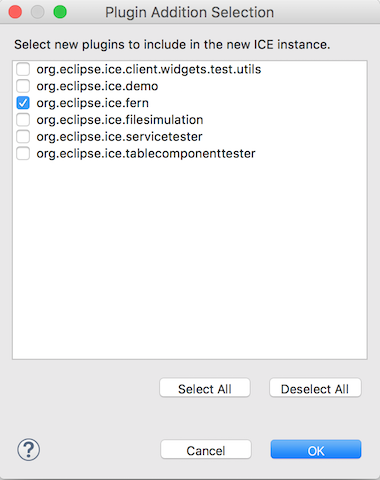
\includegraphics{figures/pluginDialog}
\end{center}
Select \texttt{org.eclipse.ice.fern} (or whatever name you chose for your
plugins) and click \texttt{OK}.
This will create and launch a new instance of ICE that includes your custom
plugins.

\subsection{Importing a Project}

This section will show you how to import existing FERN application source code
and executables into the ICE instance so that you can use it with the dashboard you
have just created. The steps are as follows:

\begin{enumerate}
\item With a new ICE instance open, close the Welcome view if necessary
\item Go to \texttt{Package Explorer} view, right click and select \texttt{New
$\rightarrow$ Synchronized C/C++ Project}

\begin{center} 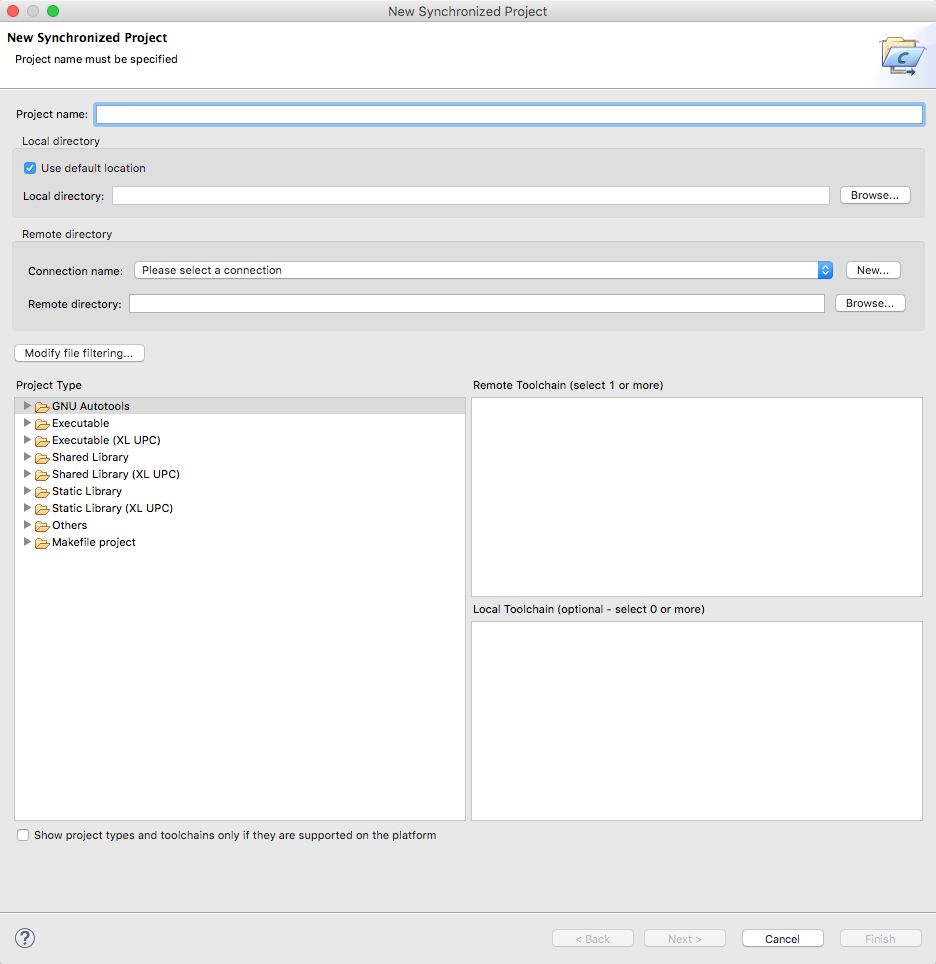
\includegraphics[width=\textwidth]{figures/newSyncWizard}
\end{center}

\item Enter \texttt{fern} for the \texttt{Project name:}
\item Click the \texttt{New\ldots} button next to the \texttt{Please select a
connection} dropdown

\begin{center} 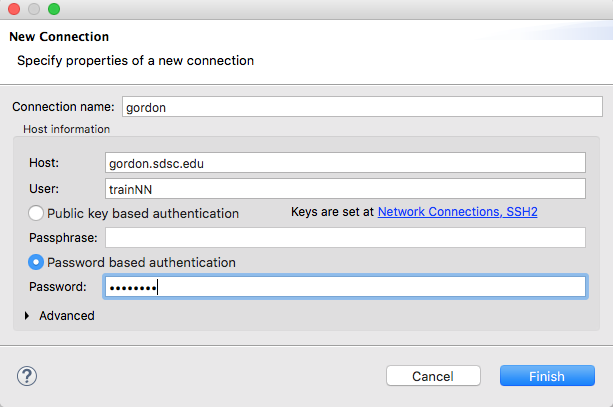
\includegraphics[width=200]{figures/newConnectionDialog}
\end{center}

\item Enter \texttt{gordon} for the \texttt{Connection name}
\item Enter \texttt{gordon.sdsc.edu} for the \texttt{Host}
\item Enter your training username for the \texttt{User}
\item Click on the \texttt{Password based authentication} button
\item Enter the training account password
\item Click \texttt{Finish}
\item Click on the \texttt{Browse\ldots} button

\begin{center} 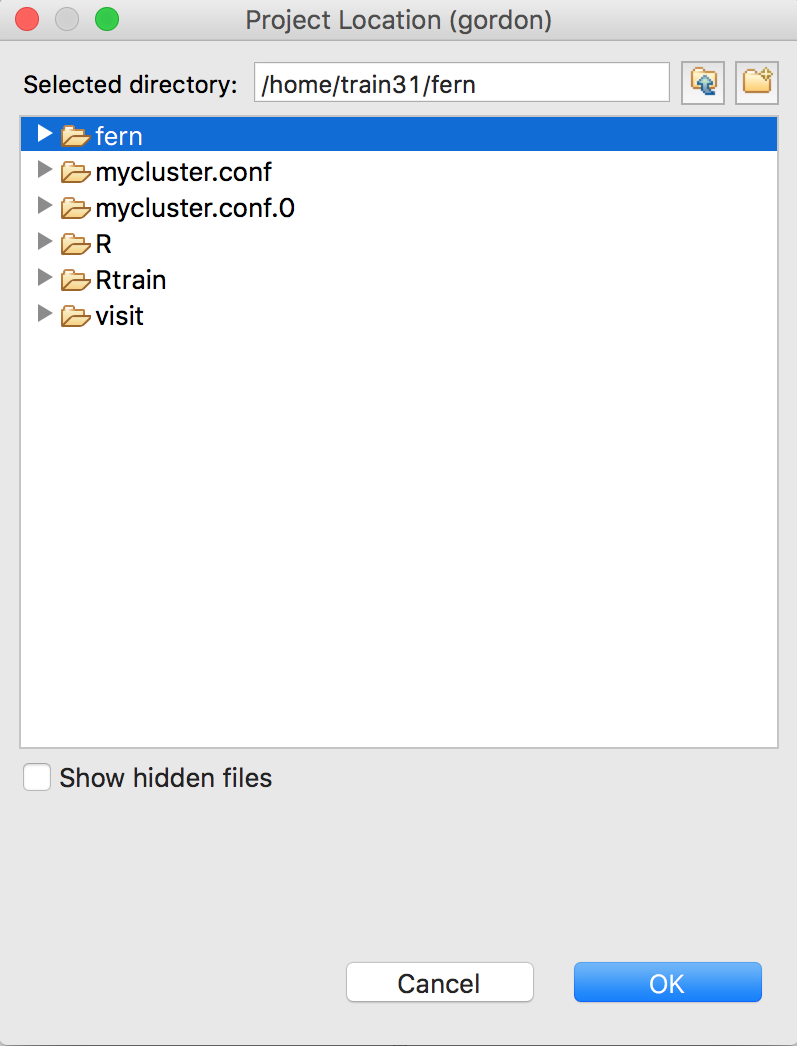
\includegraphics[width=150]{figures/dirBrowser}
\end{center}

\item Select \texttt{fern} from the directory browser and press \texttt{OK}

\begin{center} 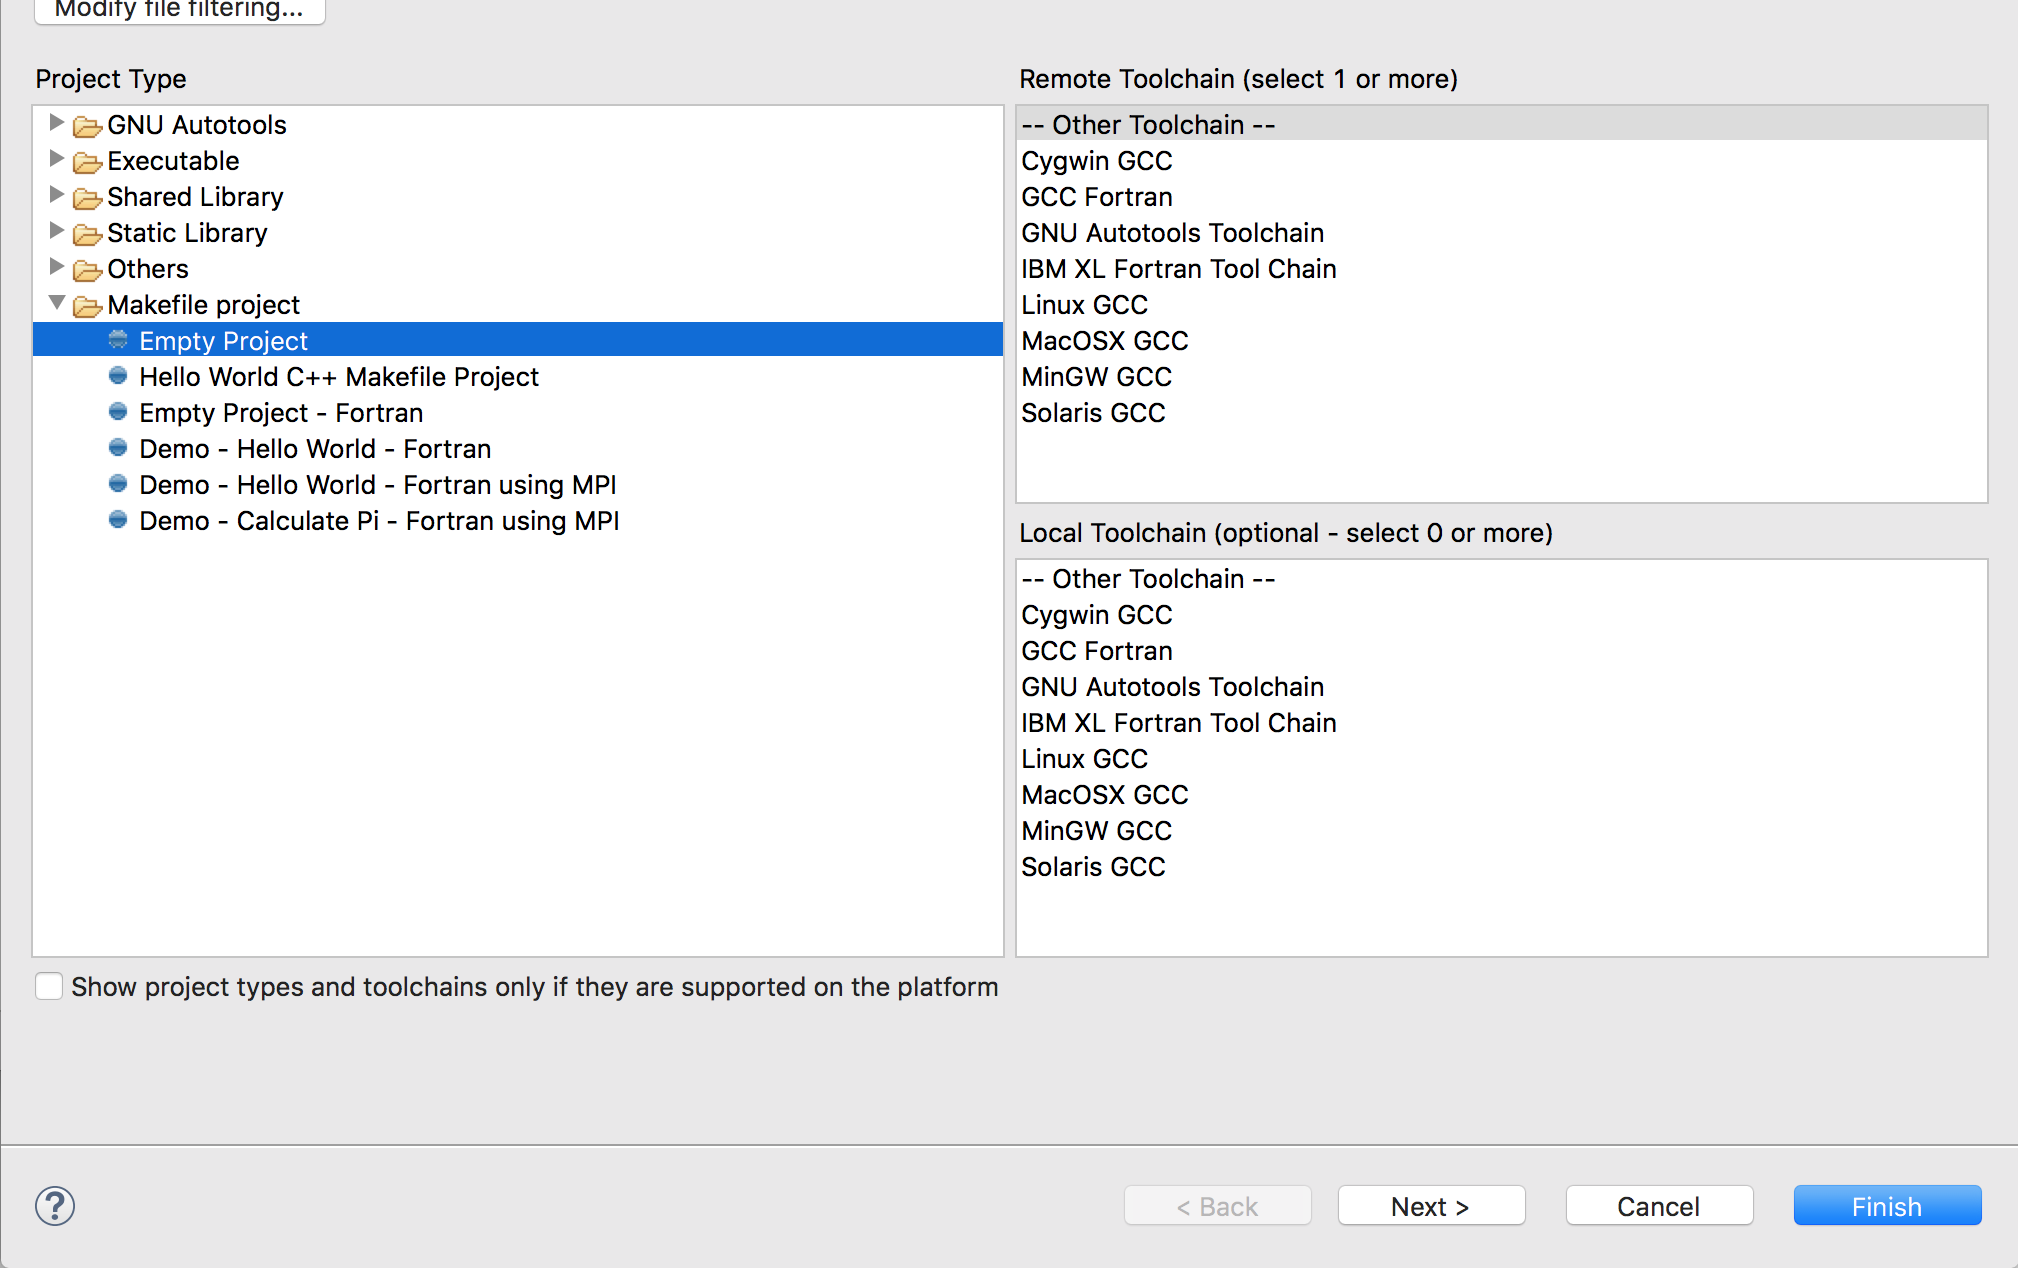
\includegraphics[width=\textwidth]{figures/projectType}
\end{center}

\item From the \texttt{Project type} section, open \texttt{Makefile project} and
choose \texttt{Empty Project}
\item Click \texttt{Finish}
\end{enumerate}

At this point you should see a \texttt{fern} project in the \texttt{Project
Explorer} view. After a few moments it should complete the synchronization
and when you open the project you will see it contains a variety of files.

\subsection{Building a Project (Optional)}

We have provided a pre-built executable in the \texttt{build} subdirectory for
the purposes of this tutorial. However if you wish to build FERN yourself, you
can proceed as follows:

\begin{enumerate}
  \item Right click on the project and select \texttt{Properties}
  \item Click on the \texttt{C/C++ Build} entry
  \item Append \texttt{build} to the end of the \texttt{Build directory} entry
  \item Click \texttt{OK}
  \item Click on the hammer icon in the toolbar
\end{enumerate}

\subsection{Creating an Input File For Your Application}

To use ICE to create an input file, you first need to instantiate the
\texttt{FernModel} you created previously. To do this, right click on the
\texttt{fern} project (the project in which you want the input file to be
located), then choose \texttt{New $\rightarrow$ Other},  select the
\texttt{Create Item Wizard}, then click on \texttt{Next>}.
\begin{center} 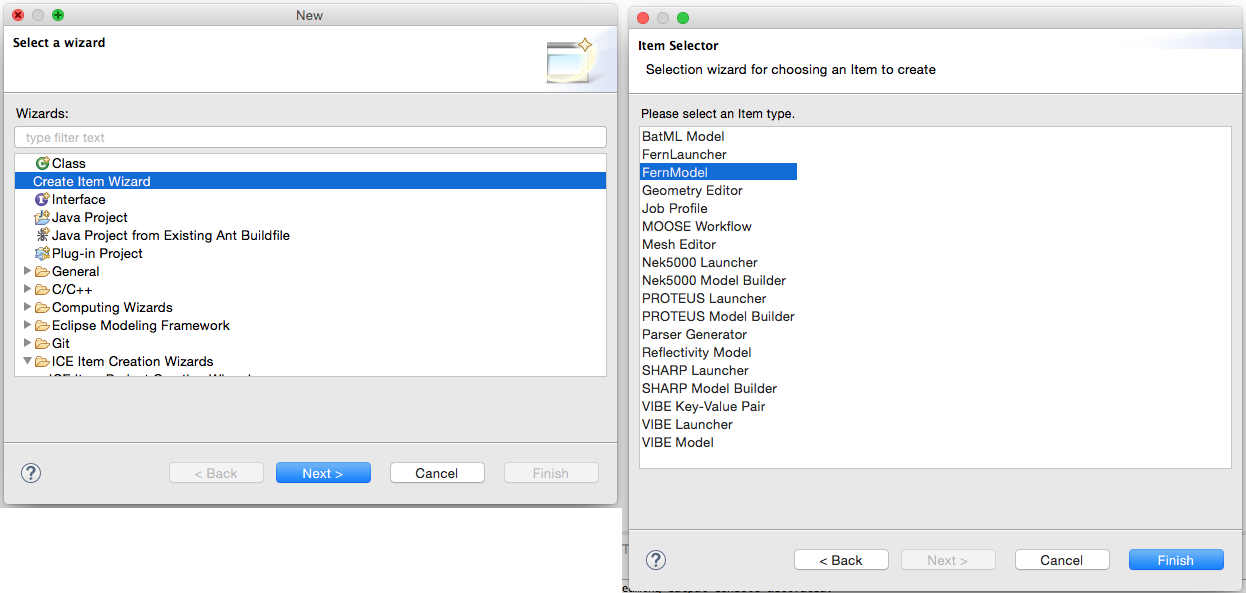
\includegraphics[width=\textwidth]{figures/creatingFernModelItem}
\end{center}
Selecting the \texttt{FernModel} Item, then click \texttt{Finish}, and you will
be presented with the view in the figure below. 
\begin{center} 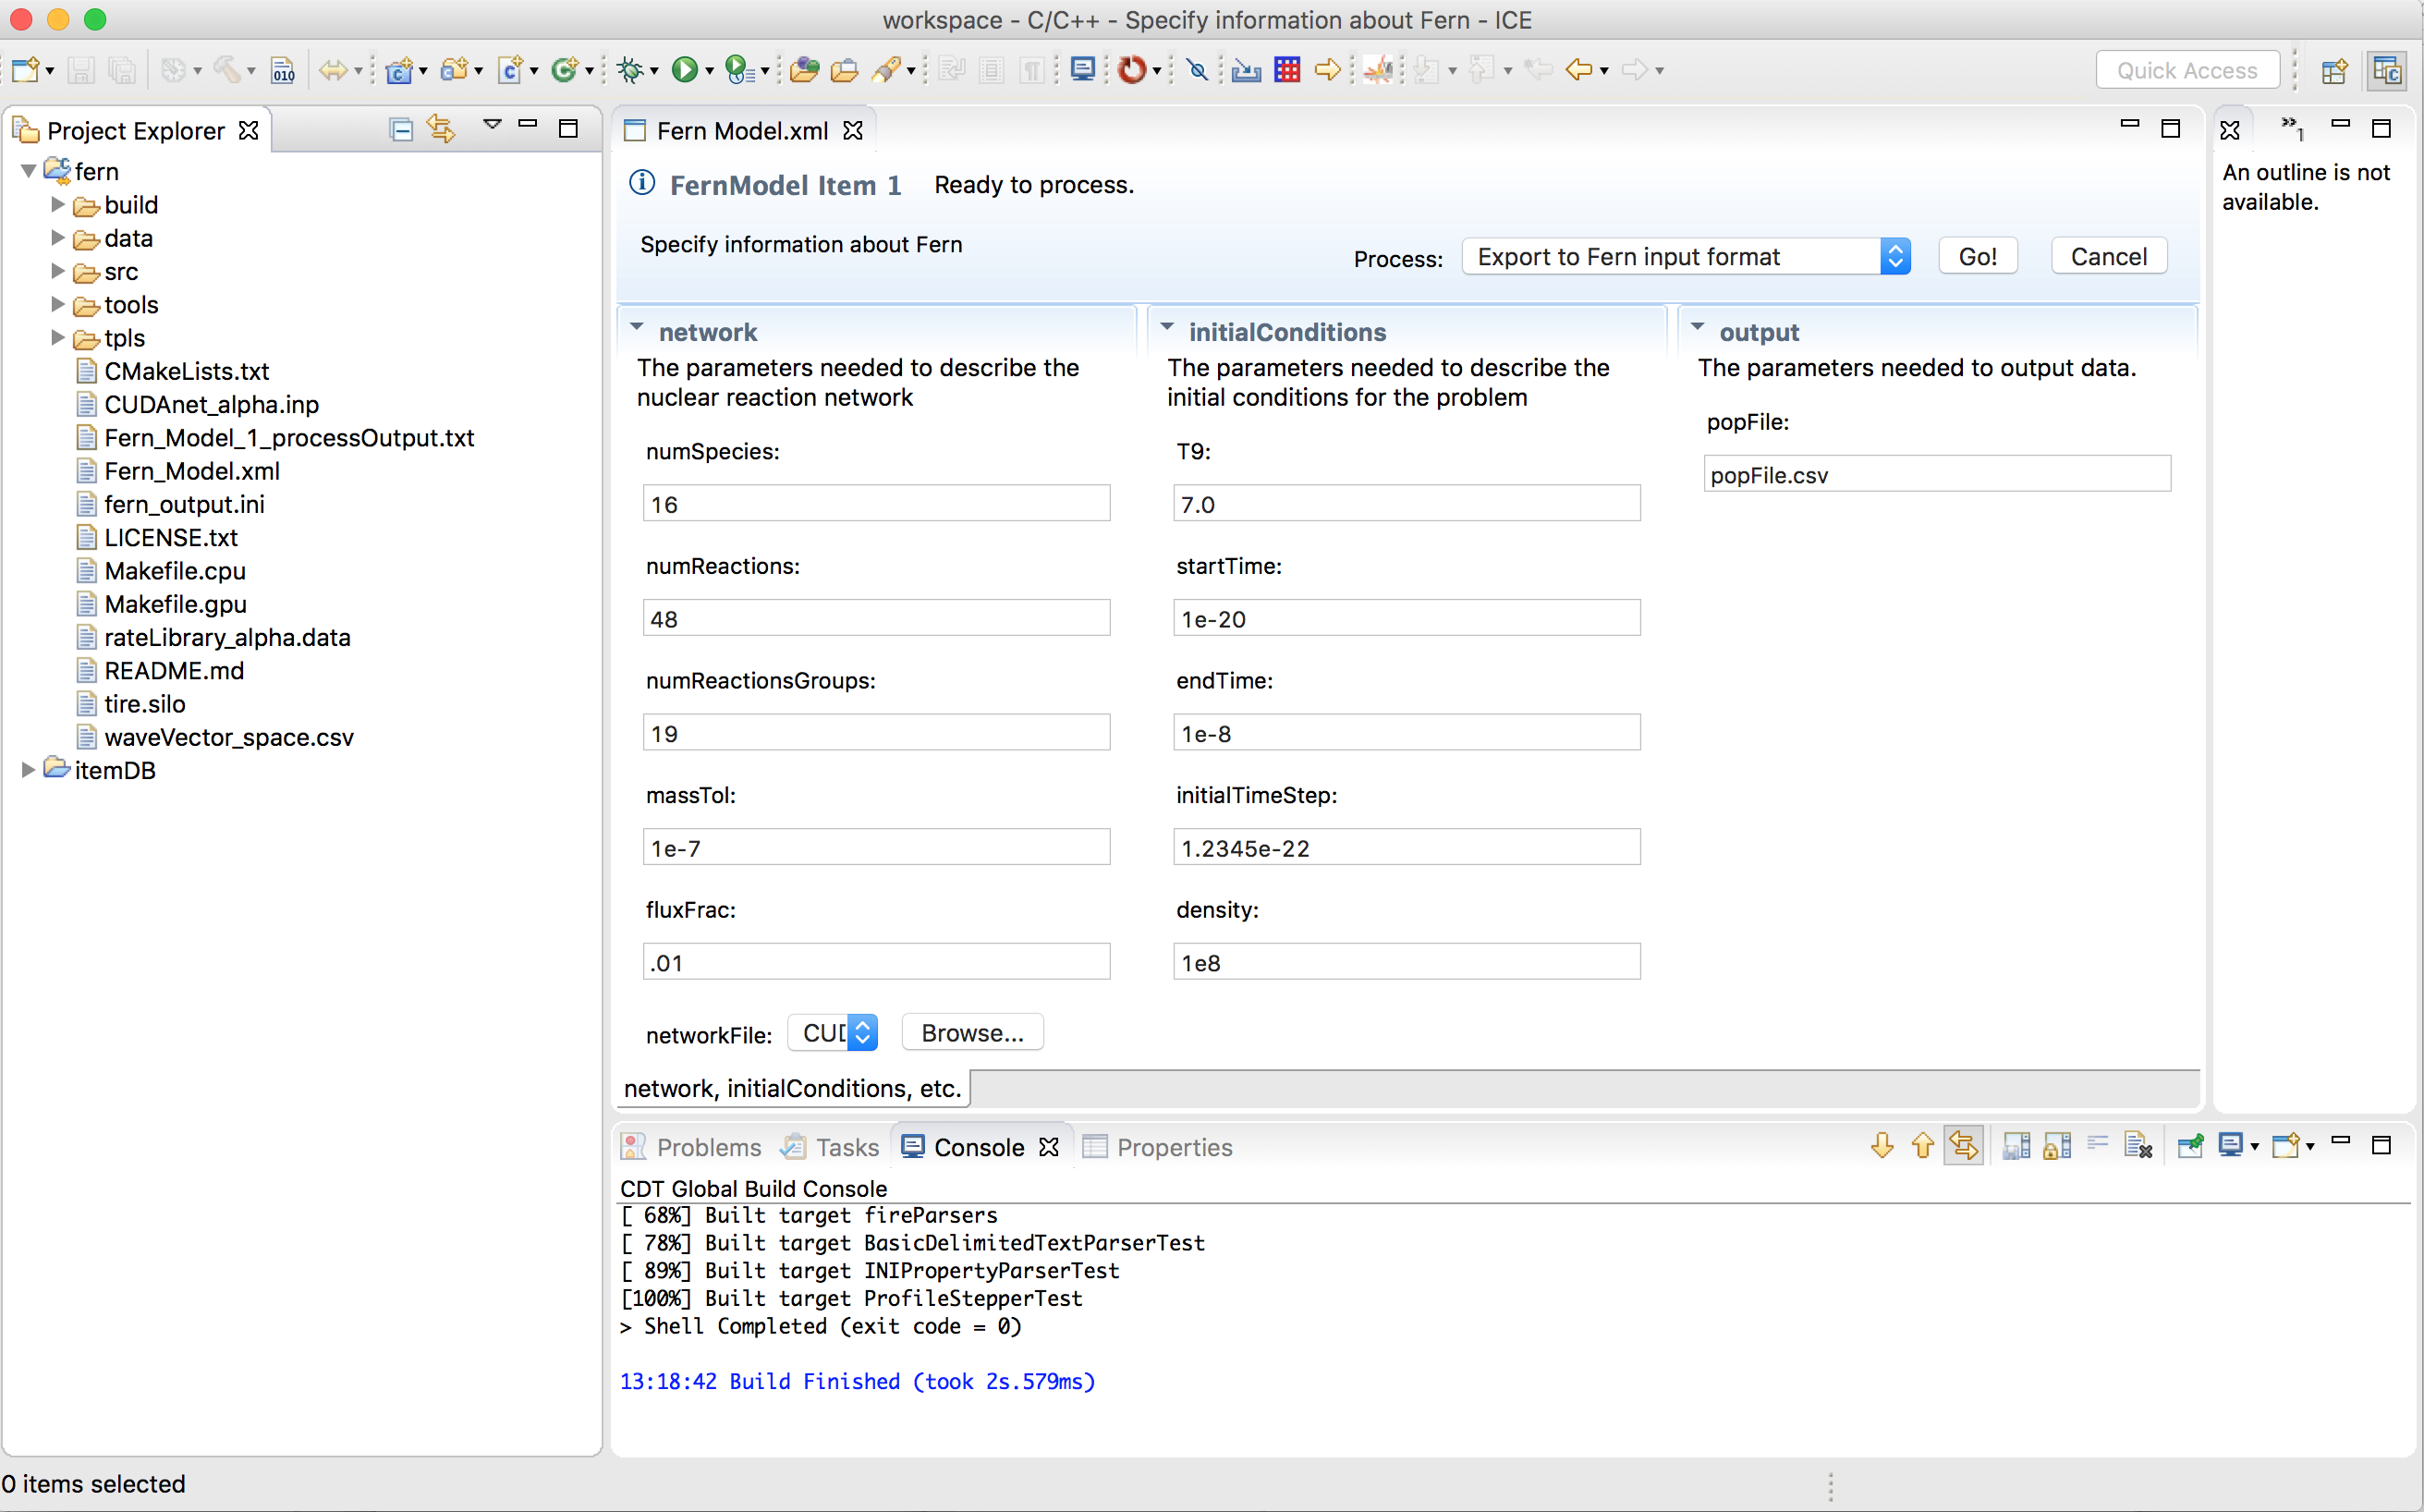
\includegraphics[width=\textwidth]{figures/fernmodelItem}
\end{center}
Here you can modify the various defaults with the values you would like for a
given Fern simulation. Once done, simply save the Item and click the
\texttt{Go!} button. This will execute the process of creating a new INI Fern
input file for use with the Fern Launcher. You can check the result by opening
the \texttt{fern\_config.ini} file, as shown below.
\begin{center} 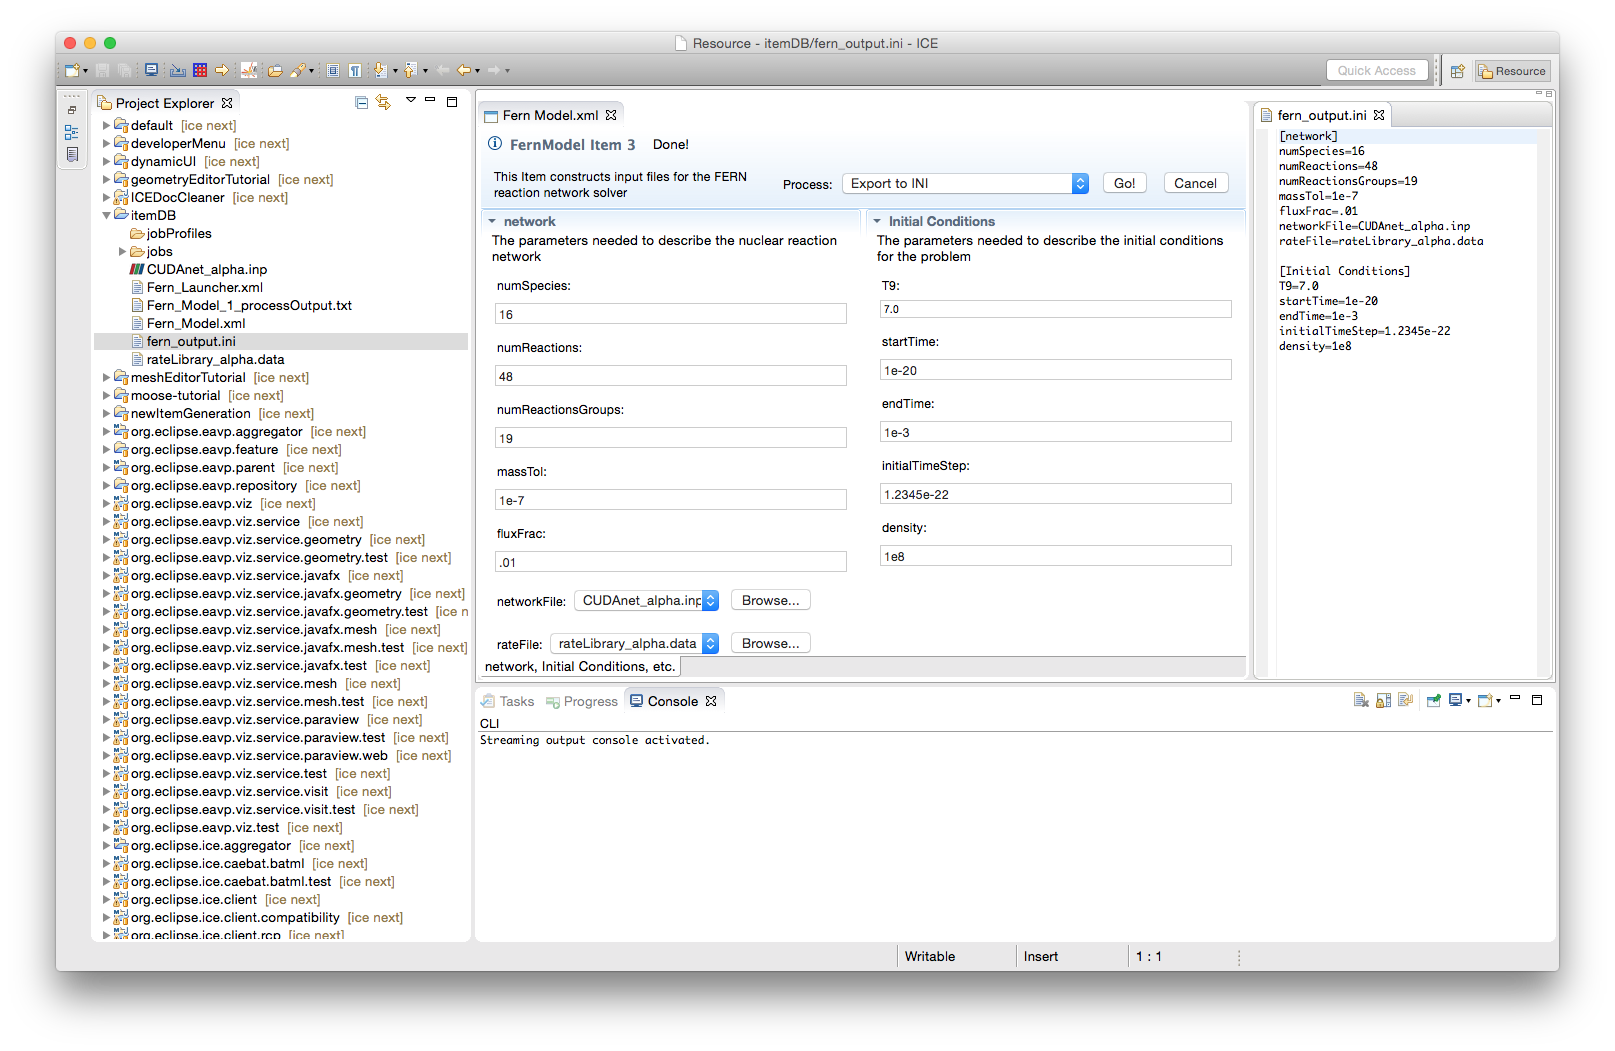
\includegraphics[width=\textwidth]{figures/result}
\end{center}

\subsection{Creating a Local Launcher}

Now you can similarly create a new FERN launcher. Note that as FERN is not
installed locally, we will not acutally launch the program using this method.

After creating the Launcher,
you should see a view like below. 
\begin{center} 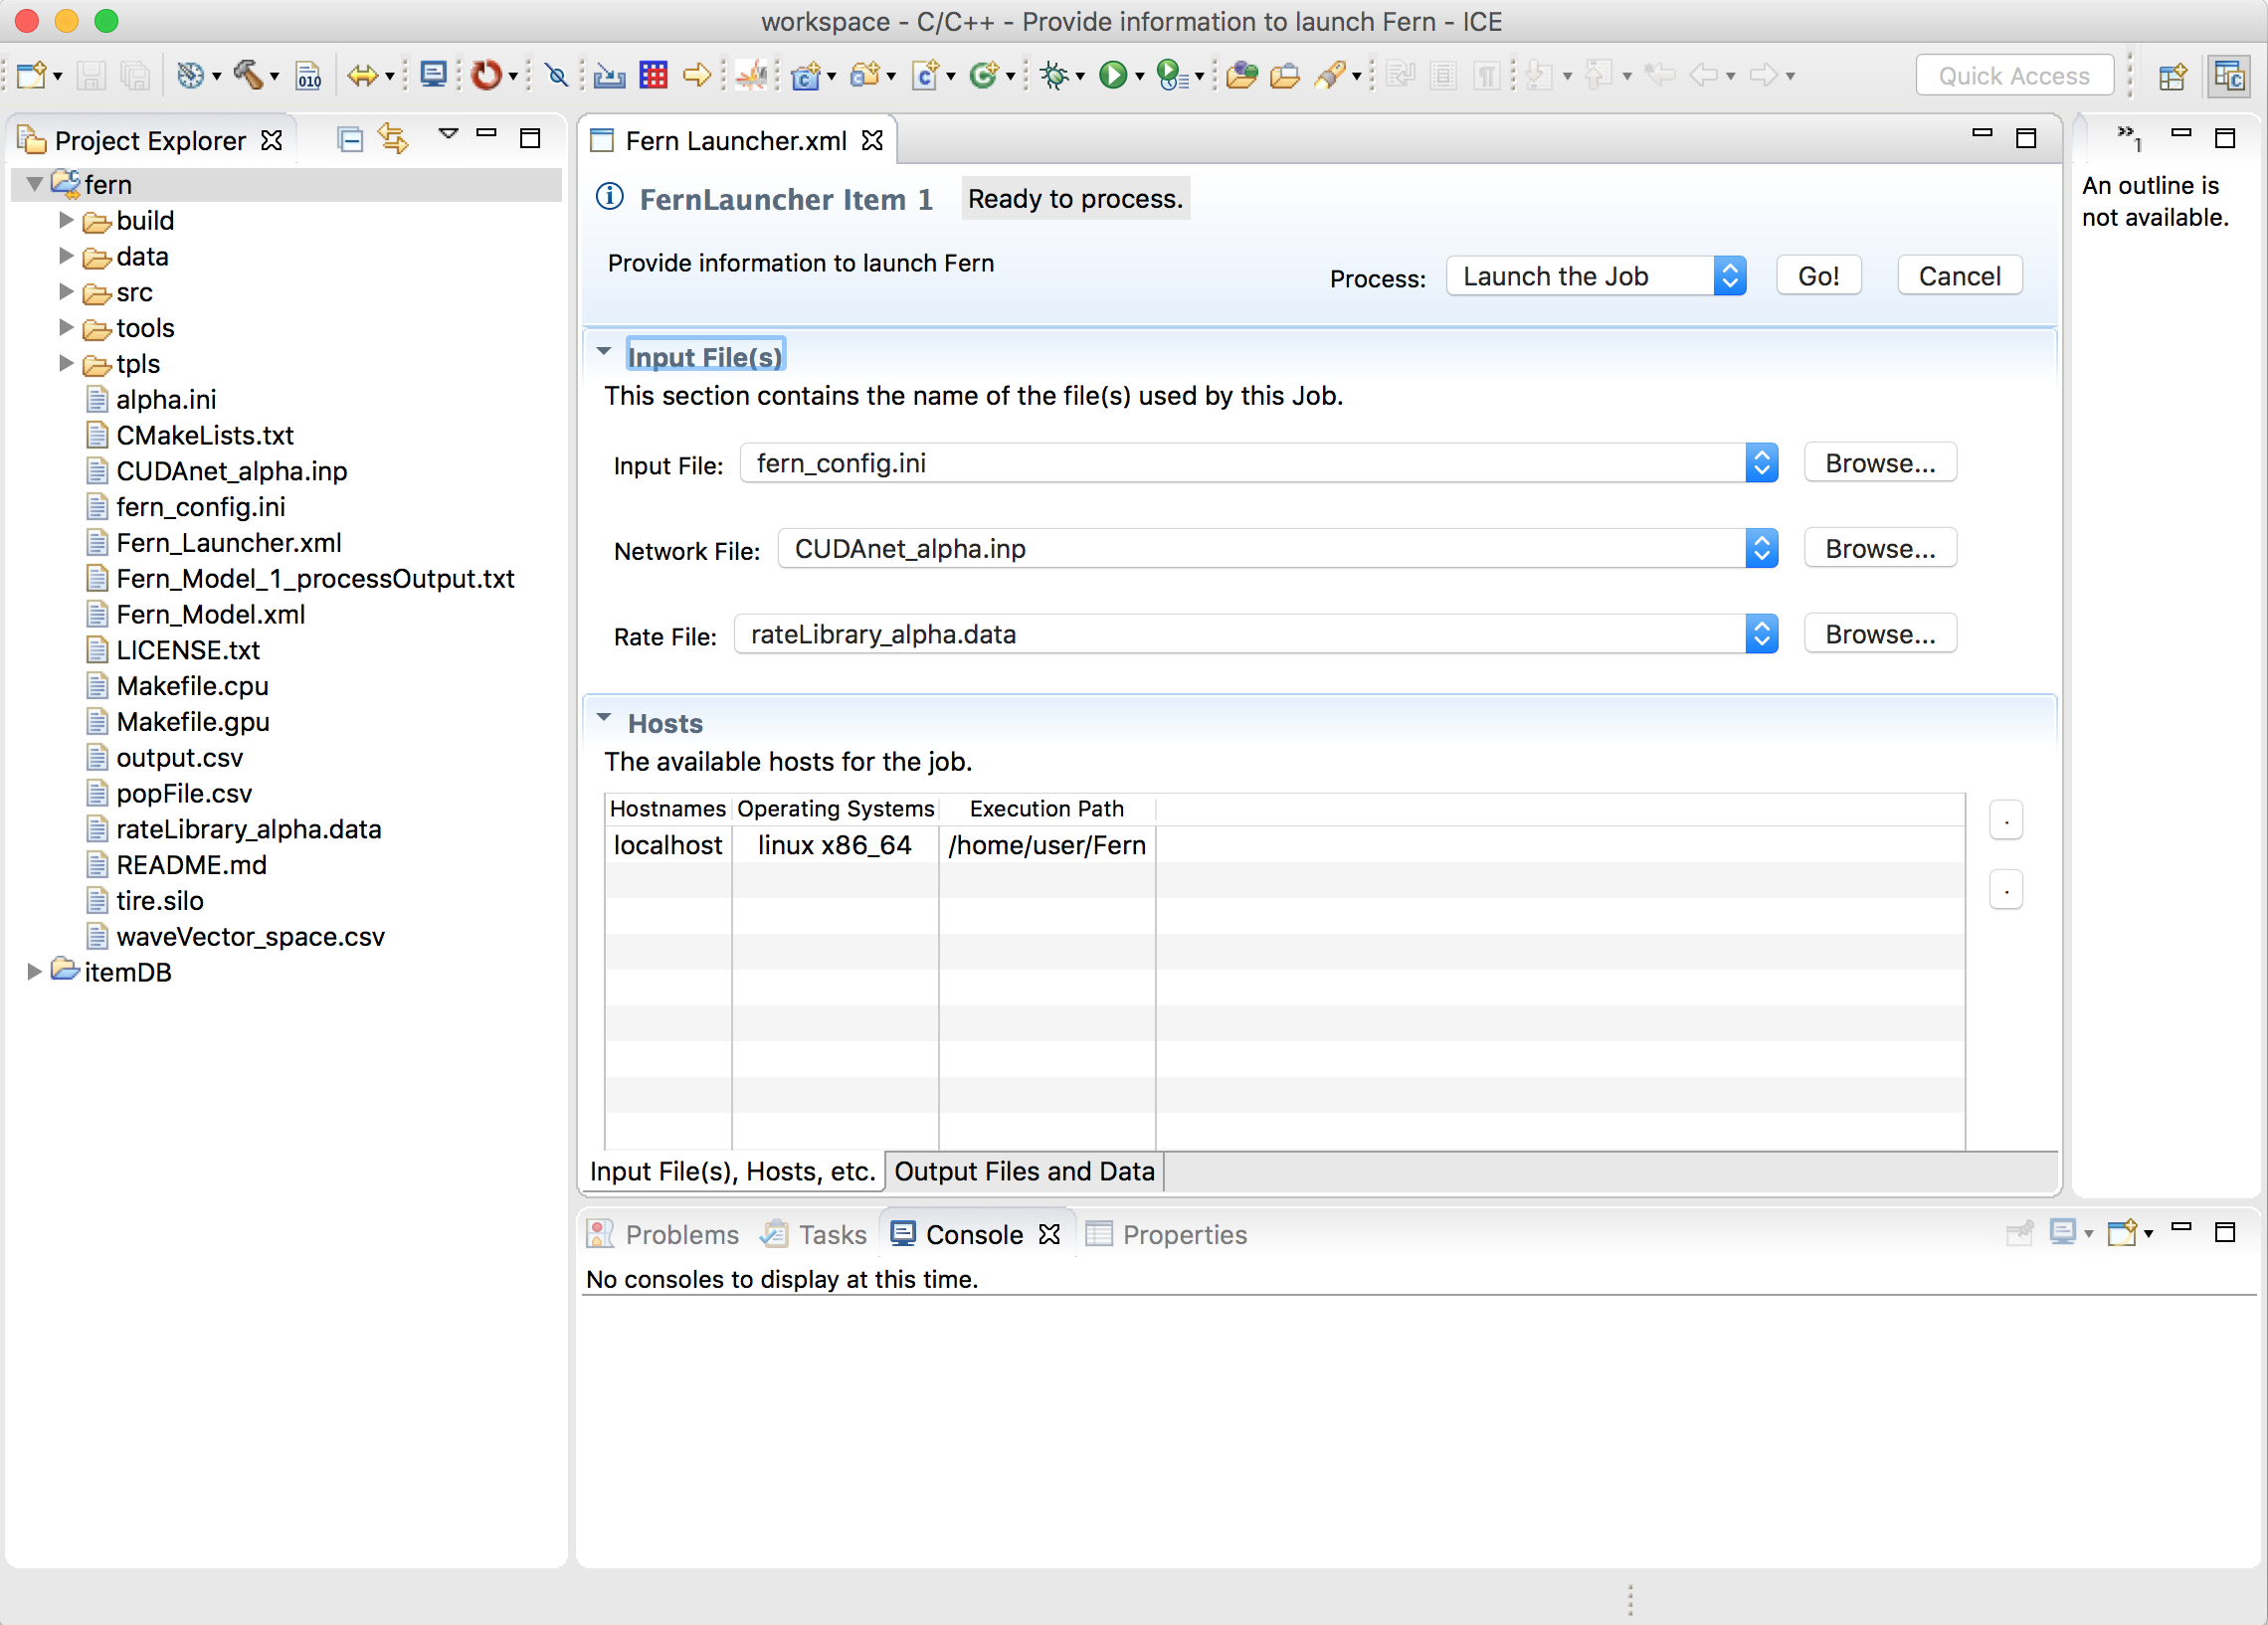
\includegraphics[width=\textwidth]{figures/launcher}
\end{center}
To configure a launch, simply set the correct
input file, along with its dependent network and rate files. 

At this point, if you had FERN built on your local machine, or if you had it
built on some remote host, you could configure that in the Hosts table. ICE
would then execute FERN based on that input. 

After the execution you should see the results in the Console, as shown below.
\begin{center} 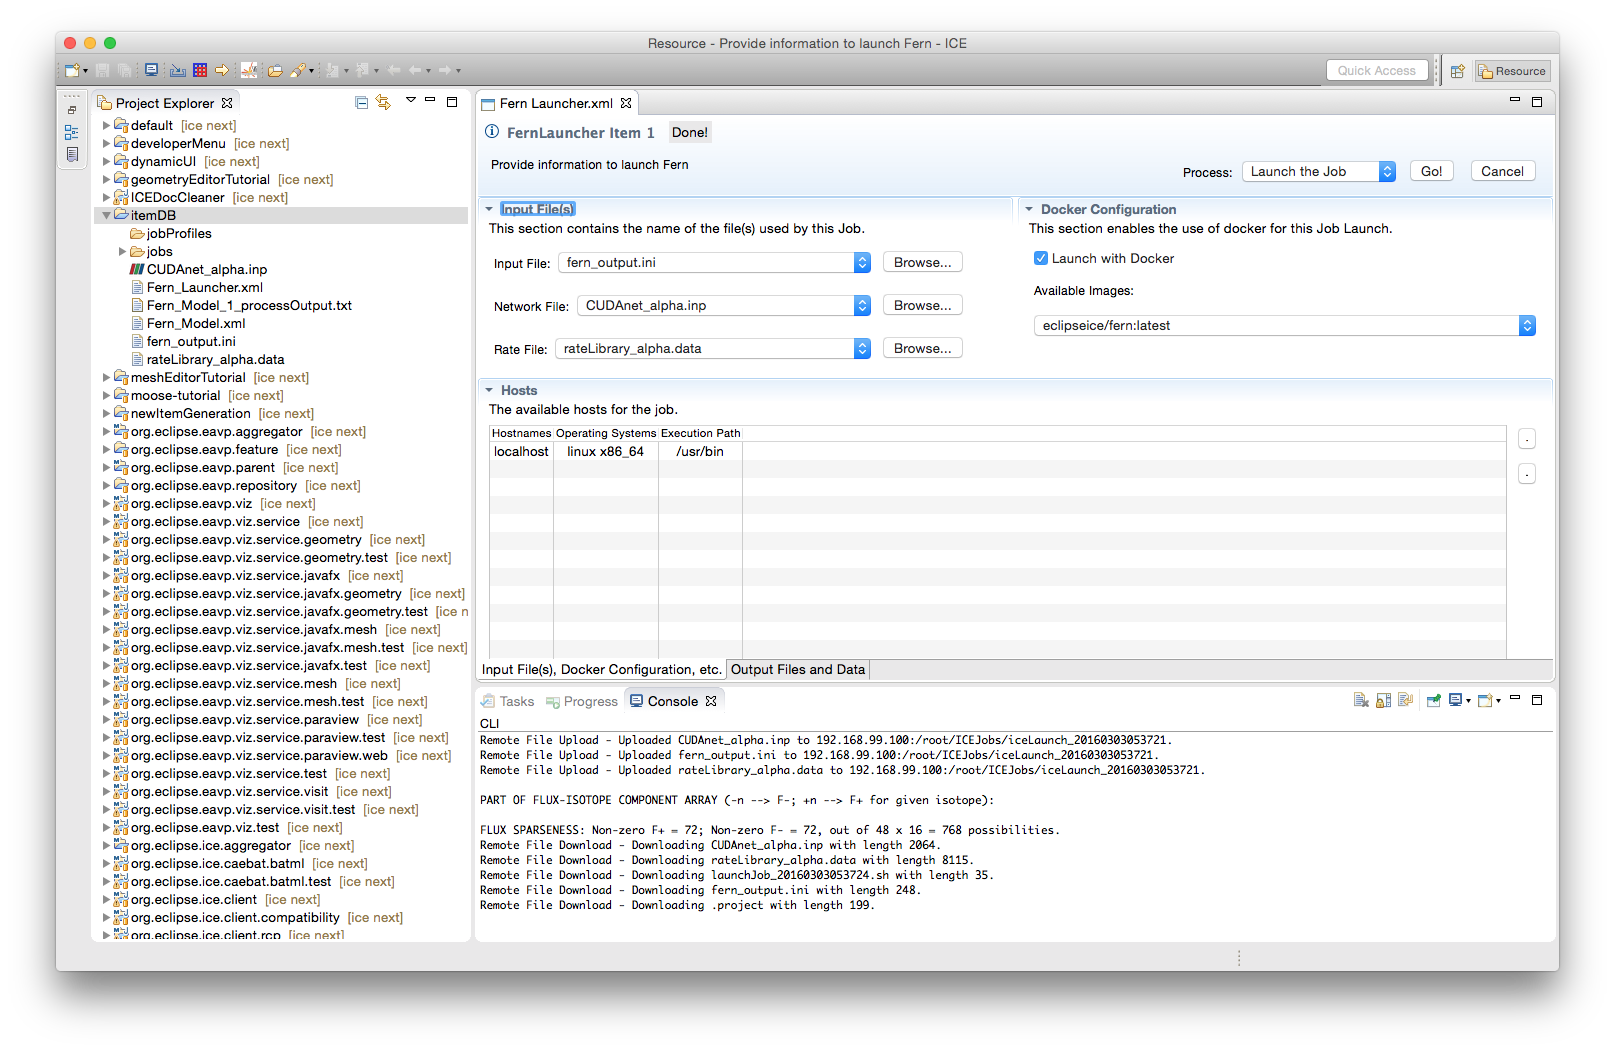
\includegraphics[width=\textwidth]{figures/launcherResult}
\end{center}
The execution should have produced a CSV file with the computed populations. You
can double-click that file to view them graphically in the ICE Plot Editor. 

\subsection{Creating a Remote Launcher}

Launching FERN remotely involves creating a \textit{Parallel launch
configuration}.
This procedure is not yet integrated with the ICE launcher, but will be
available in the next release of ICE.

A Parallel launch configuration for your application is created as follows:

\begin{enumerate}
  \item Select the \texttt{Run $\rightarrow$ Run Configurations\ldots} menu
  \item Click on the \texttt{Parallel Application} entry, then click the
  \texttt{New} button
  \item From the \texttt{Target System Configuration} dropdown, select
  \texttt{Generic Torque Batch}
  \item From the \texttt{Please select a connection}, choose the \texttt{gordon}
  connection you created earlier
  \item Click \texttt{Yes} when asked if you would like to run a command on the
  remote system (optionally check the box to not ask again)
  \item After a few seconds, you should see the job submission form
  \item Select \texttt{normal} for the queue
  
  \begin{center} 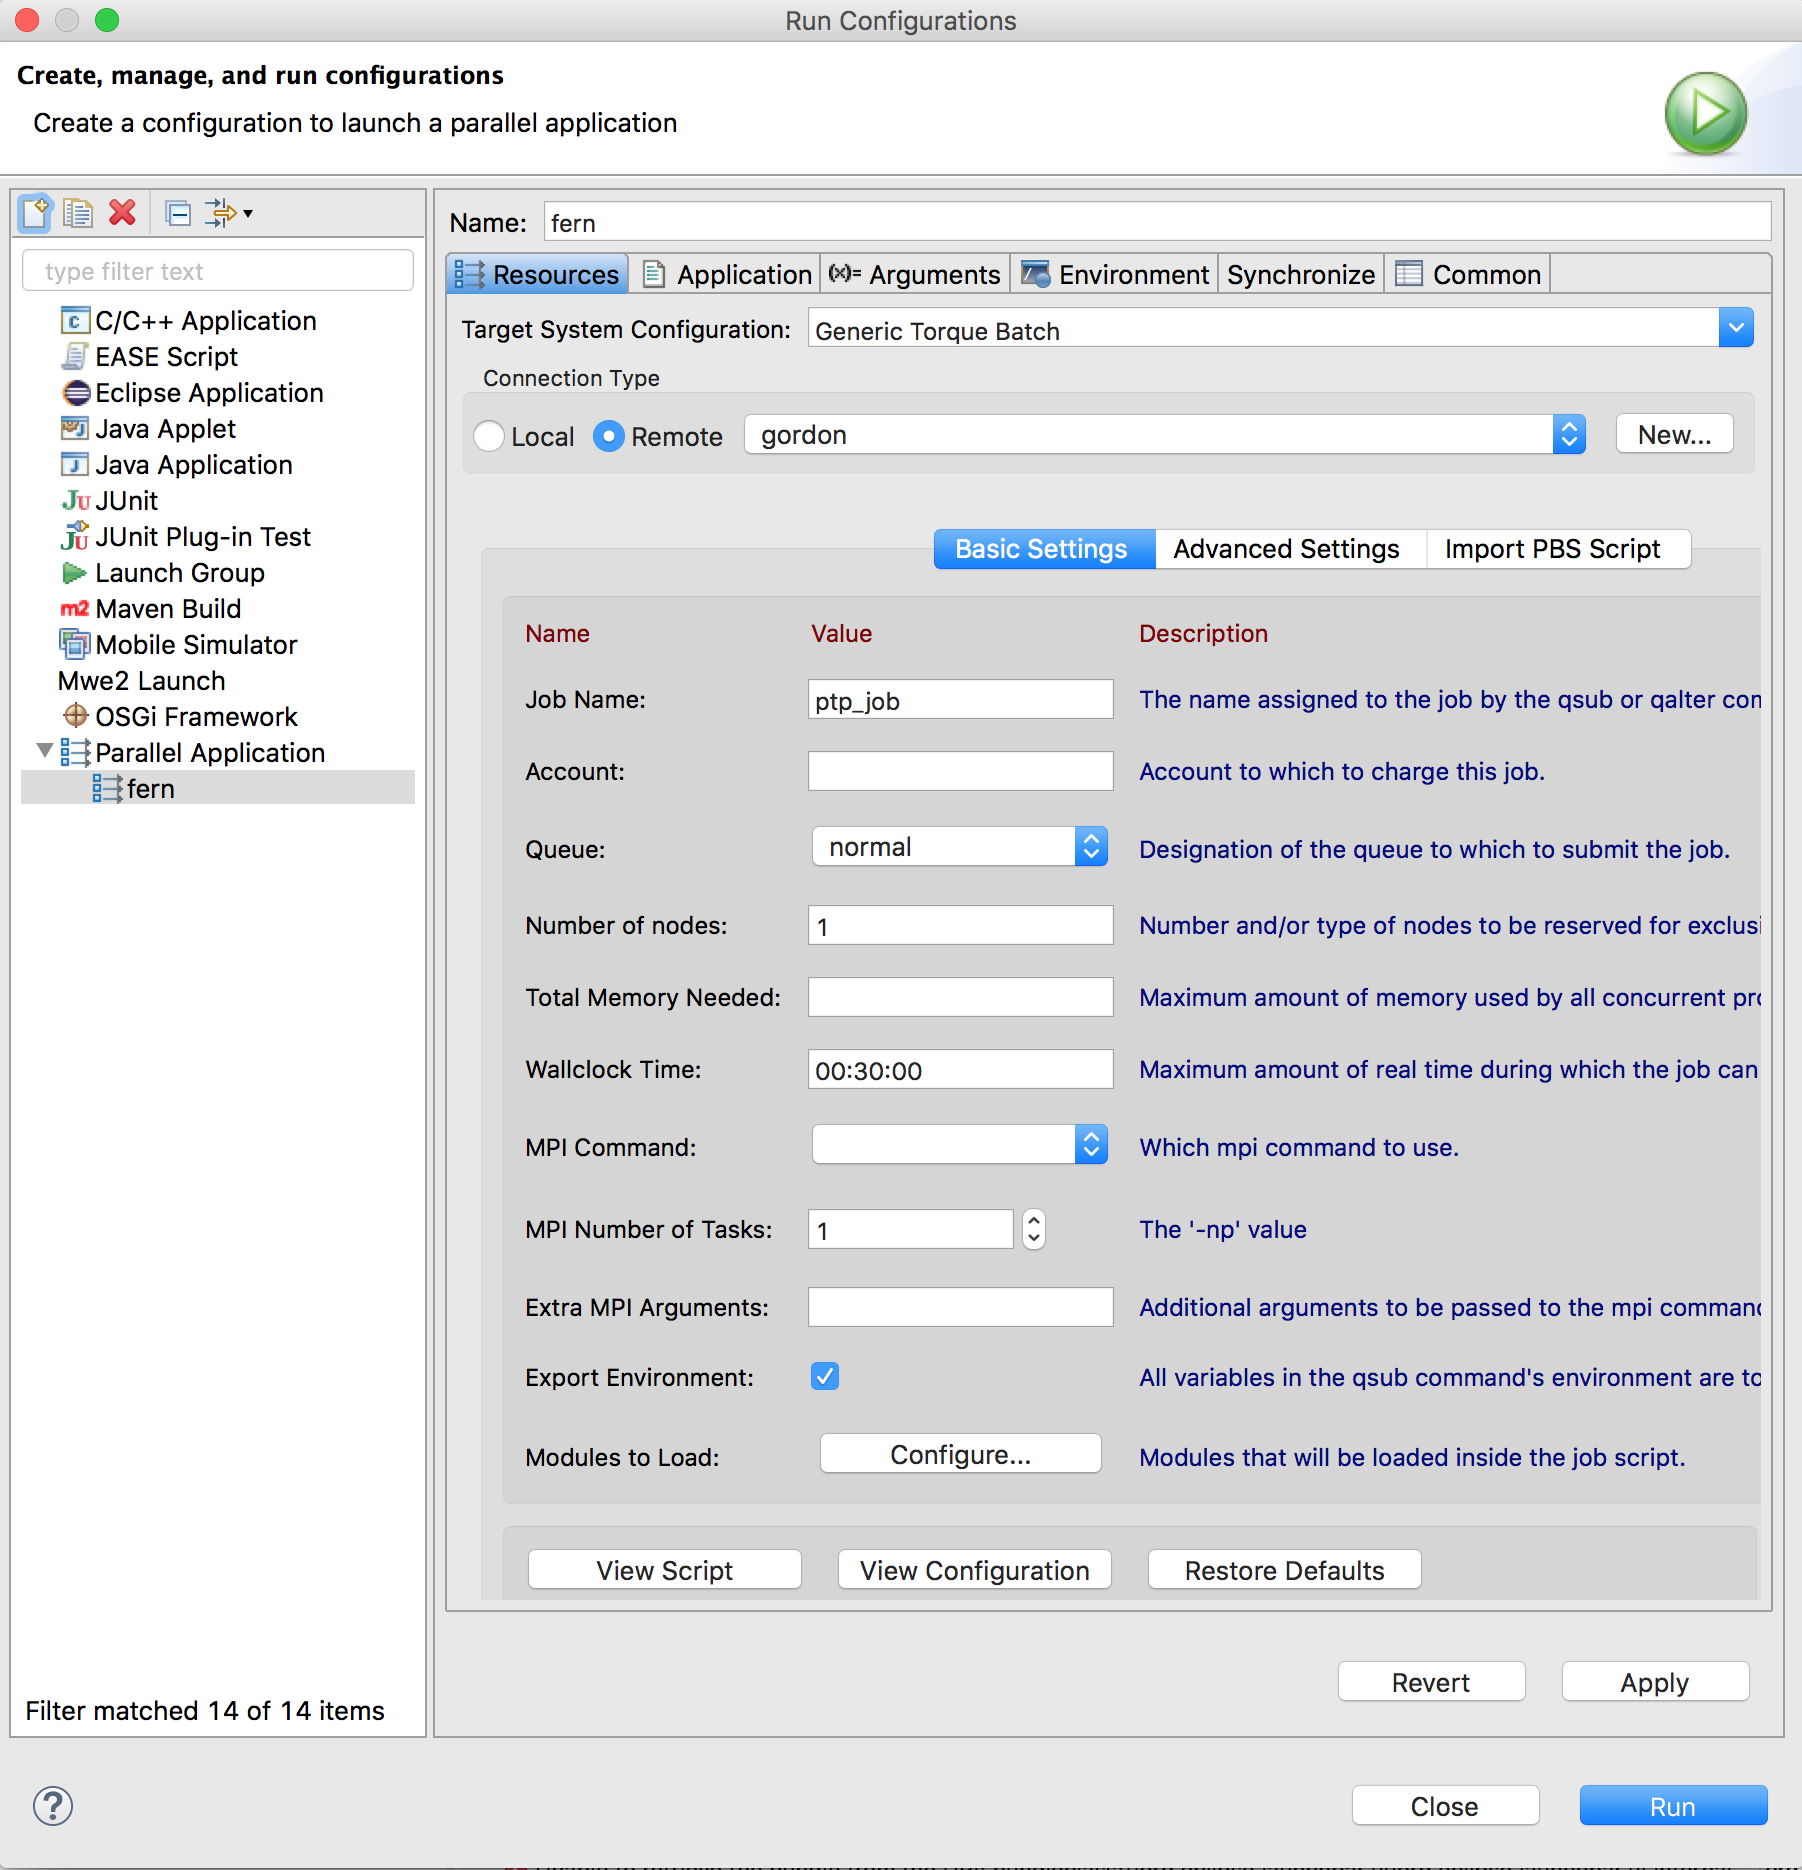
\includegraphics[width=\textwidth]{figures/runConfiguration}
  \end{center}
  
  \item Switch to the \texttt{Application} tab
  \item If the project field doesn't contain anything, click \texttt{Browse} and
  choose the \texttt{fern} project
  \item Click \texttt{Browse} next to the \texttt{Application program} field,
  open the \texttt{build} directory, select \texttt{fern-exec}, then click
  \texttt{OK}
  
  \begin{center} 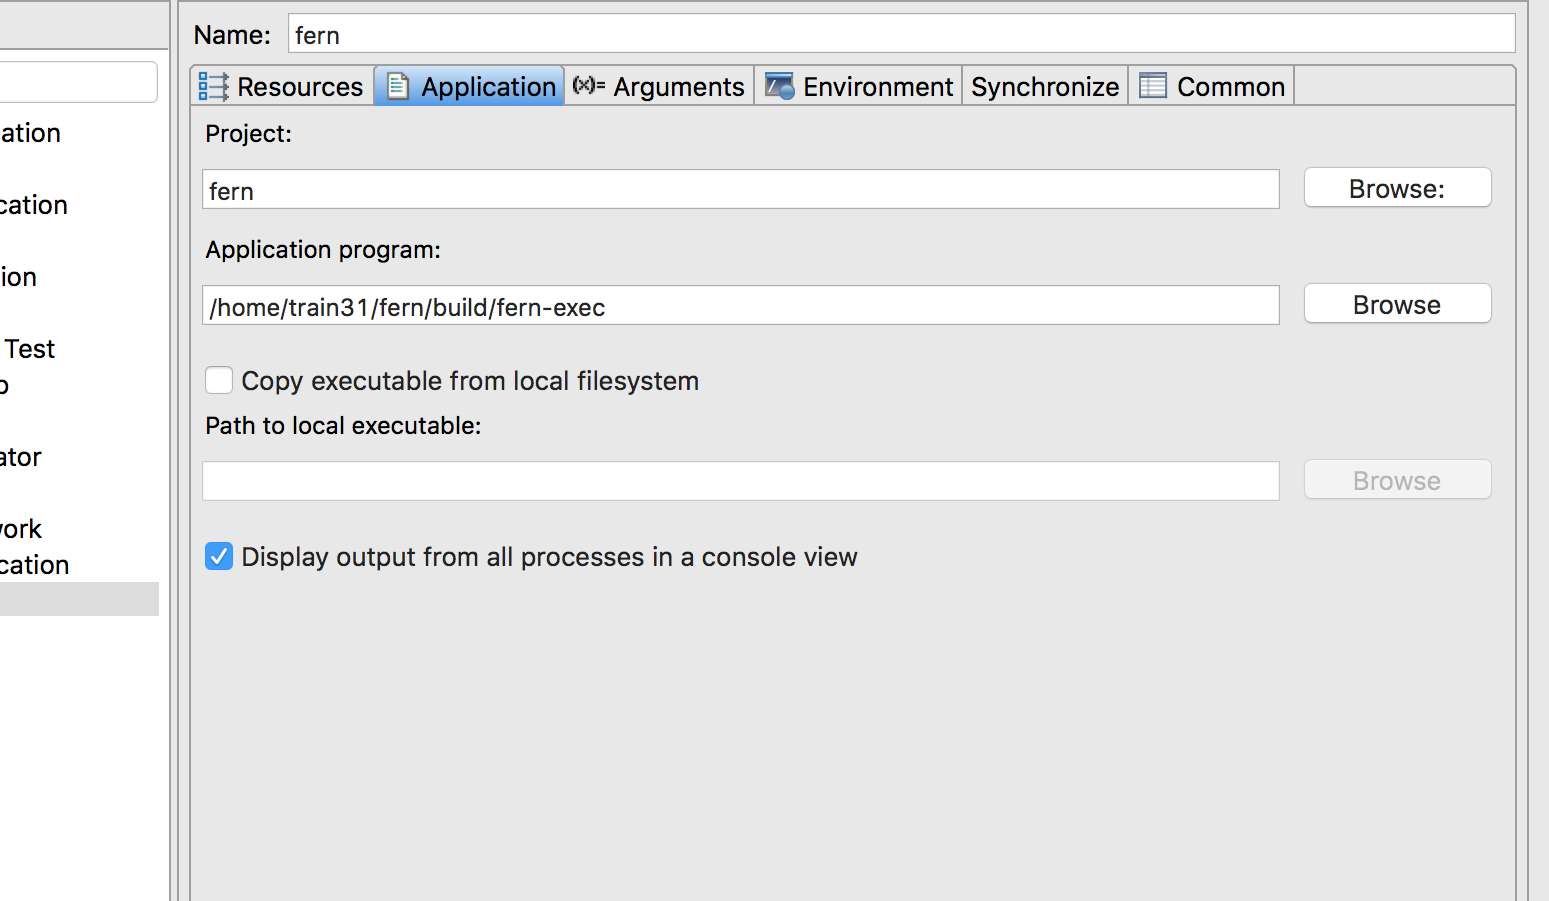
\includegraphics[width=300]{figures/applicationTab}
  \end{center}
  
  \item Switch to the \texttt{Arguments} tab and enter the name of the
  outputfile you chose in the \texttt{FernModel} file
  \item Uncheck \texttt{Use default working directory}
  
  \begin{center} 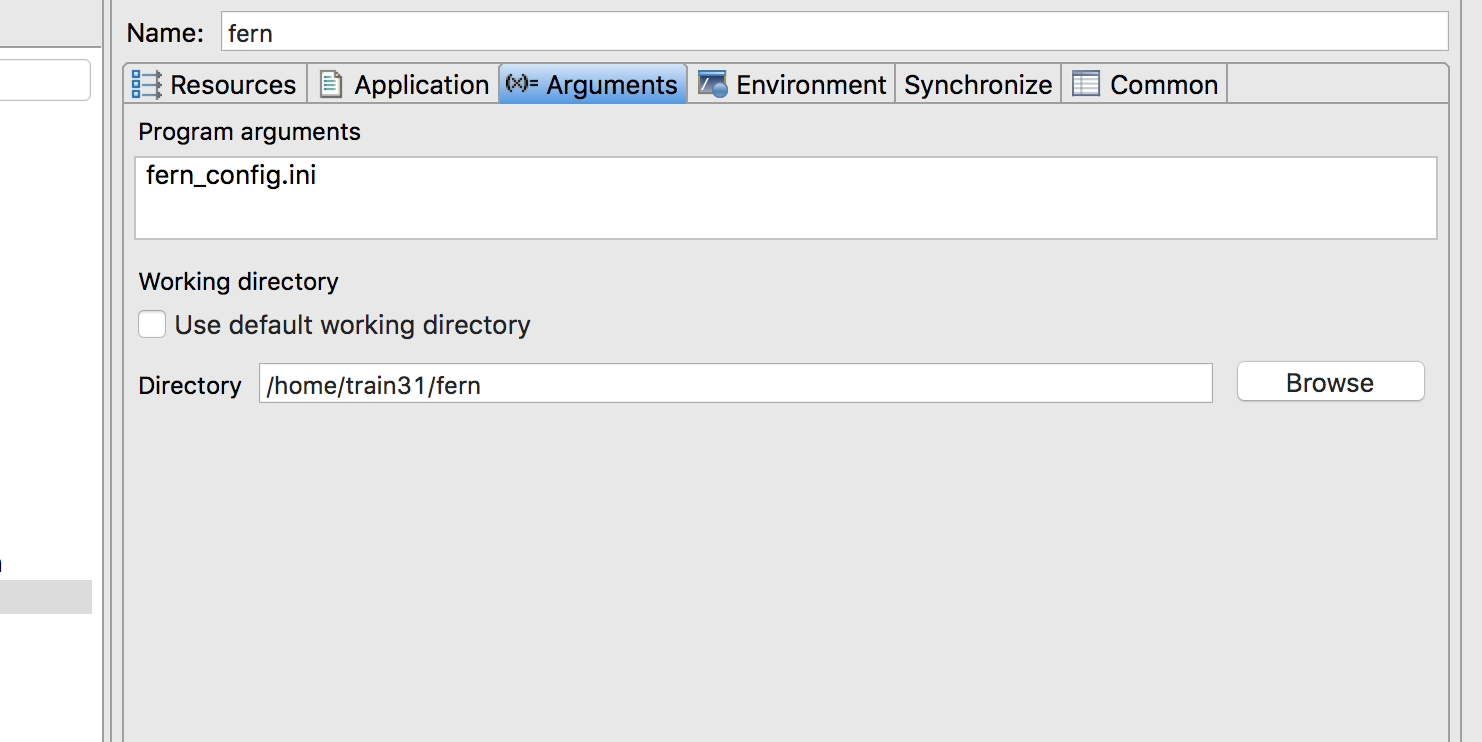
\includegraphics[width=300]{figures/argumentsTab}
  \end{center}
  
  \item Click \texttt{Run} to submit the job 
\end{enumerate}

During the job submission, you will be asked if you would like to switch to the
\texttt{System Monitoring} perspecive. Click \texttt{Yes} to see this feature.
The image belows shows a typical instance of this perspective in action.

\begin{center} 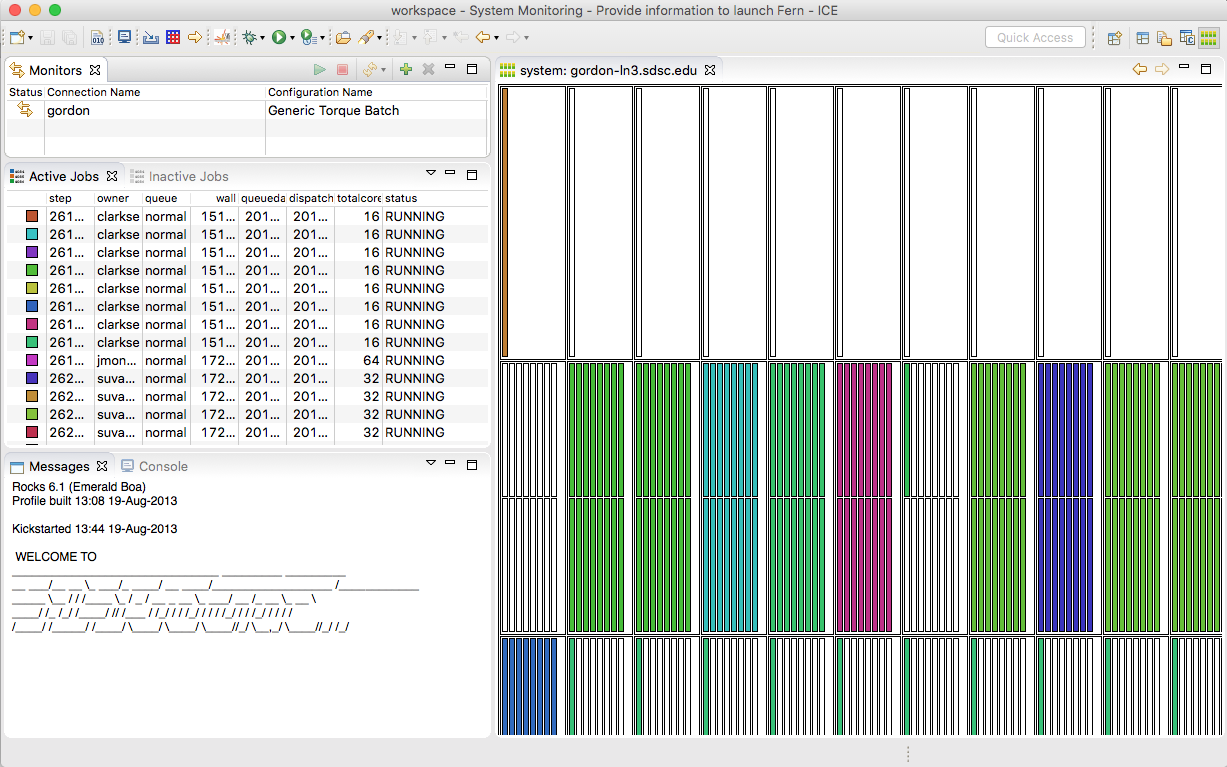
\includegraphics[width=\textwidth]{figures/sysMon}
\end{center}

Click on the \texttt{Inactive Jobs} view and scroll to the bottom. You should
see a job from your username that is either submitted or completed. When the job
is completed, you can switch back to the \texttt{C/C++ Perspective}.

\begin{center} 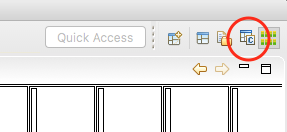
\includegraphics[width=200]{figures/cppPersp}
\end{center}

In the \texttt{Project Explorer} view, click on the \textit{synchronize}
button to copy the output files back to your local machine. 

\begin{center} 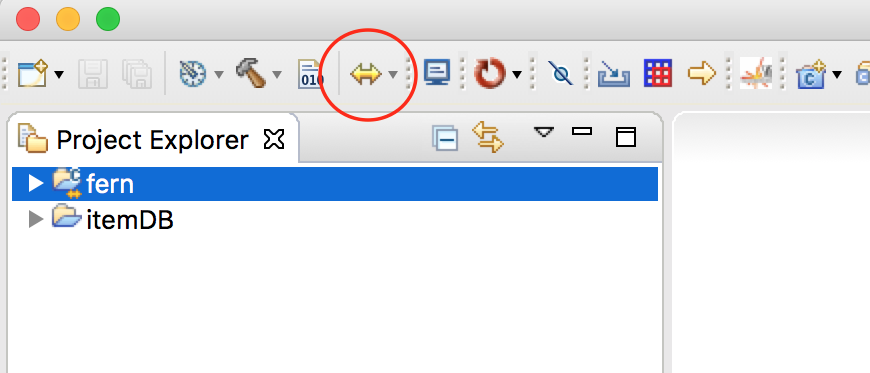
\includegraphics[width=200]{figures/syncButton}
\end{center}

If the project is not already open, you can open it now and
you should see the resulting CSV file. Double click on this file to launch the CSV viewer.

